\documentclass[12pt]{article}
%%% ========== Package setup ==========
\usepackage{listings}   % Script listing package
\usepackage{wrapfig}    % Wrap Figure or table package
\usepackage{multicol}   % Multicolumn package
\usepackage{pdfpages}   % Include pdf files

%%% ========== Format setup ==========
%% Setup chinese words encoder
\usepackage{xeCJK}
\XeTeXlinebreaklocale "zh"
\XeTeXlinebreakskip = 0pt plus 1pt

%% More word fonts
\usepackage{fontspec}
\setmainfont{Times New Roman}
\renewcommand{\familydefault}{\rmdefault}
\setCJKmainfont{標楷體}

%% Chinese paragraph format
\usepackage{indentfirst}
\setlength{\parindent}{2em}

%% Page margin
\usepackage[a4paper, total={6in,8in}]{geometry}

%%% ========== Document ==========
\begin{document}

\newcommand{\MakeTitlePage}[1]{
\begin{titlepage}
    \begin{center}

        \fontsize{50}{10}
        \selectfont
        Optimal Control

        \vspace{1cm}

        \fontsize{30}{10}
        \selectfont
        Final exam

        \vspace{11cm}

        \begin{tabular}{ r l }
            班級: & 航太四A \\ [10pt]
            姓名: & 吳柏勳 \\ [10pt]
            學號: & 407430635 \\ [10pt]
            座號: & 3 \\ [10pt]
        \end{tabular}

    \end{center}
\end{titlepage}
}
\MakeTitlePage{5}
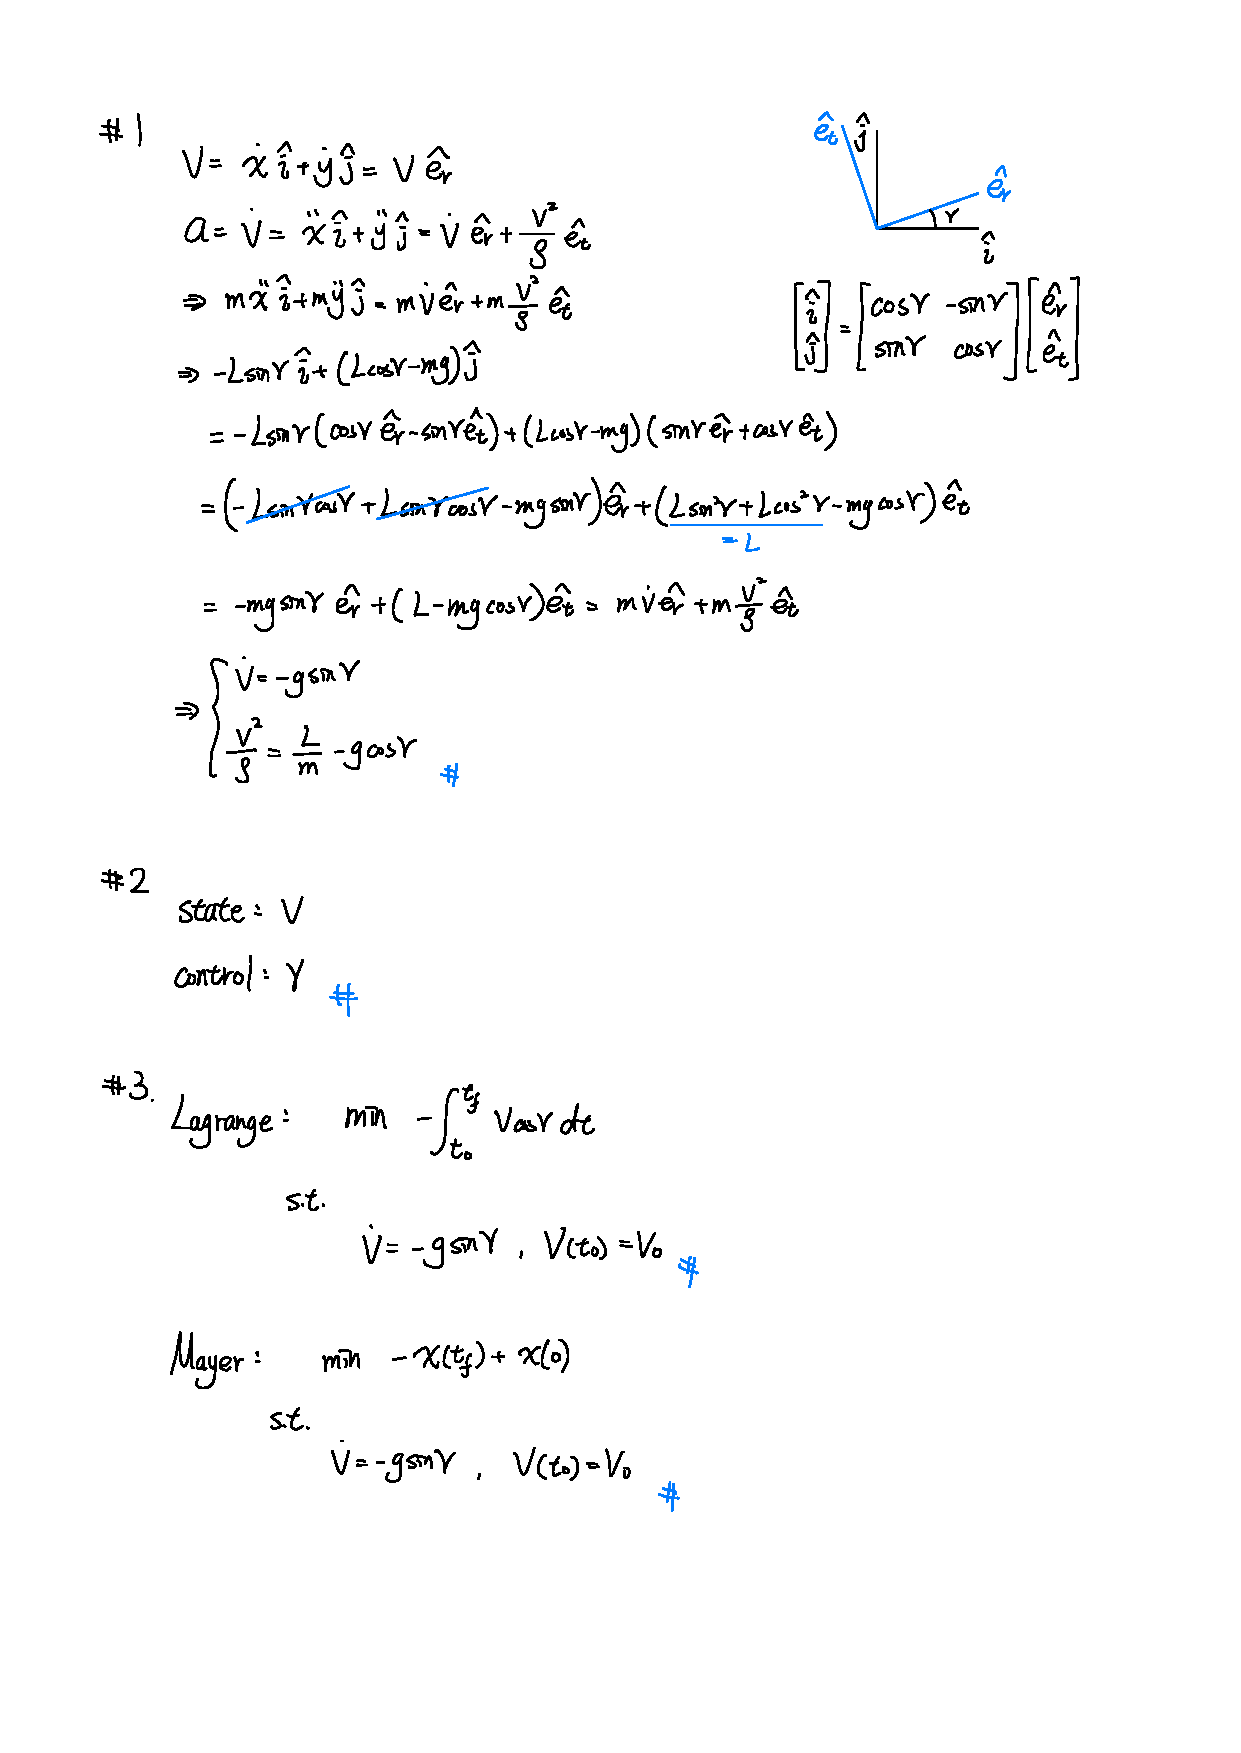
\includepdf[pages=-]{handout.pdf}

\subsection*{\#6}

\begin{verbatim}
    clear;clc;close all
    [time, state] = ode45(@ode, [0 10], [0; 0; 10; 0]);

    figure(); hold on
    plot(state(:,1), state(:,2))
    grid on
    xlabel("x"); ylabel("y")

    function dstate = ode(~, state)
    % Parameter define:
    %   - state: [x; y; V; gamma]

    g = 9.81;
    dx = state(3)*cosd(state(4));
    dy = state(3)*sind(state(4));

    dstate = [dx; dy; -g*sind(state(4)); g*cosd(state(4))/state(3)];
    end
\end{verbatim}

\centering
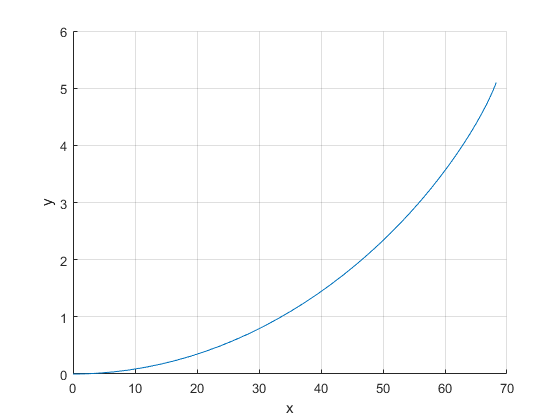
\includegraphics [width=4in]{HW5_01.png}



\end{document}
